% Copyright (c) 2022 Alexander Bluhm <bluhm@openbsd.org>
%
% Permission to use, copy, modify, and distribute this software for any
% purpose with or without fee is hereby granted, provided that the above
% copyright notice and this permission notice appear in all copies.
%
% THE SOFTWARE IS PROVIDED "AS IS" AND THE AUTHOR DISCLAIMS ALL WARRANTIES
% WITH REGARD TO THIS SOFTWARE INCLUDING ALL IMPLIED WARRANTIES OF
% MERCHANTABILITY AND FITNESS. IN NO EVENT SHALL THE AUTHOR BE LIABLE FOR
% ANY SPECIAL, DIRECT, INDIRECT, OR CONSEQUENTIAL DAMAGES OR ANY DAMAGES
% WHATSOEVER RESULTING FROM LOSS OF USE, DATA OR PROFITS, WHETHER IN AN
% ACTION OF CONTRACT, NEGLIGENCE OR OTHER TORTIOUS ACTION, ARISING OUT OF
% OR IN CONNECTION WITH THE USE OR PERFORMANCE OF THIS SOFTWARE.

\documentclass[14pt,aspectratio=169]{beamer}
%\usepackage[nomixage,puffy]{genuaslides}
\usetheme{Frankfurt}
\usepackage{tikz}
\usetikzlibrary{positioning}
\usetikzlibrary{shapes.geometric}
\usepackage{adjustbox}
\usepackage{graphicx}
\graphicspath{gnuplot}
\usepackage{multirow}

\author{Alexander Bluhm}
\title{Faster OpenBSD Networking}
\institute{bluhm@openbsd.org}
\date{EuroBSDCon, September 2022}

\begin{document}

\begin{frame}
\titlepage
\end{frame}

\begin{frame}{Agenda}
\setcounter{tocdepth}{1}
\tableofcontents
\end{frame}

\section{Overview}

\subsection{Network Layers}
\begin{frame}{Network Layers}
\begin{itemize}
\item syscall
\item file descriptor
\item socket
\item IP protocol
\item IPsec
\item IP input, output, forwarding
\item pf
\item routing, ARP, ND6
\item interface
\item driver
\item hardware
\end{itemize}
\end{frame}

\subsection{Other Layers}
\begin{frame}{Other Layers}
\begin{itemize}
\item interrupts
\item malloc, pools
\item tasks
\item multicast
\item ifconfig ioctl
\item pseudo devices:
    aggr bpe bridge carp egre enc eoip etherip gif gre lo mgre mpe
    mpip mpw nvgre pair pflog pflow pfsync ppp pppoe svlan tap tpmr
    trunk tun veb vether vlan vport vxlan wg
\end{itemize}
\end{frame}

\subsection{Developement}
\begin{frame}{Developement}
\begin{itemize}
\item ideal
    \begin{itemize}
    \item make it MP safe
    \item run in parallel
    \item make it fast
    \item advance in steps
    \end{itemize}
\item reality
    \begin{itemize}
    \item work on whatever makes fun
    \item deal with 40 years old code
    \end{itemize}
\end{itemize}
\end{frame}

\subsection{History}
\begin{frame}{History}
\begin{itemize}
\item interrupts with spl
\item kernel lock
\item kernel threads
\item MP safe subsystems
\item netlock
\item multiqueue NIC
\item shared netlock
\end{itemize}
\end{frame}

\section{Kernel Context}

\subsection{Single Processor}
\begin{frame}{Single Processor}
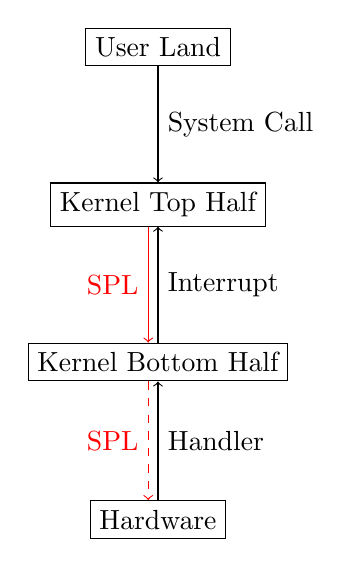
\begin{tikzpicture}
    \path (0, 2) node [draw] (ul) {User Land};
    \path (0, 0) node [draw] (to) {Kernel Top Half};
    \draw [->] (ul) -- (to) node[midway,right] {System Call};
    \path (0, -2) node [draw] (bo) {Kernel Bottom Half};
    \draw [<-] (to.south) -- (bo.north) node[midway,right] {Interrupt};
    \path (to.south) node (tos) {} (bo.north) node (bon) {};
    \draw [->,red] (tos.west) -- (bon.west) node[midway,left,red] {SPL};
    \path (0, -4) node [draw] (hw) {Hardware};
    \draw [<-] (bo) -- (hw) node[midway,right] {Handler};
    \path (bo.south) node (bos) {} (hw.north) node (hwn) {};
    \draw [->,red,dashed] (bos.west) -- (hwn.west) node[midway,left,red] {SPL};
\end{tikzpicture}
\end{frame}

\subsection{Multi Processor Kernel Lock}
\begin{frame}{Multi Processor Kernel Lock}
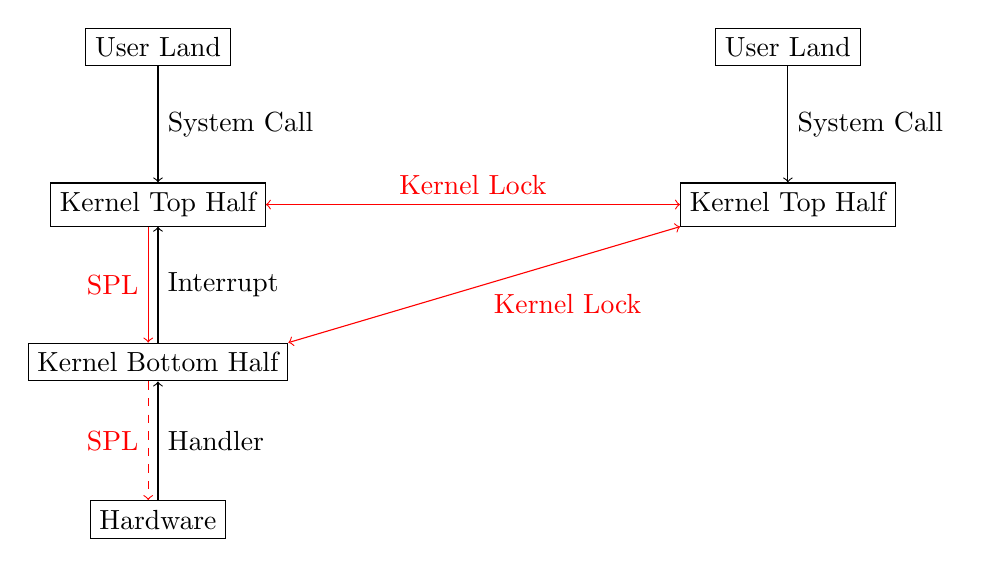
\begin{tikzpicture}
    \path (0, 2) node [draw] (ul) {User Land};
    \path (0, 0) node [draw] (to) {Kernel Top Half};
    \draw [->] (ul) -- (to) node[midway,right] {System Call};
    \path (0, -2) node [draw] (bo) {Kernel Bottom Half};
    \draw [<-] (to.south) -- (bo.north) node[midway,right] {Interrupt};
    \path (to.south) node (tos) {} (bo.north) node (bon) {};
    \draw [->,red] (tos.west) -- (bon.west) node[midway,left,red] {SPL};
    \path (0, -4) node [draw] (hw) {Hardware};
    \draw [<-] (bo) -- (hw) node[midway,right] {Handler};
    \path (bo.south) node (bos) {} (hw.north) node (hwn) {};
    \draw [->,red,dashed] (bos.west) -- (hwn.west) node[midway,left,red] {SPL};

    \path (8, 2) node [draw] (ul1) {User Land};
    \path (8, 0) node [draw] (to1) {Kernel Top Half};
    \draw [->] (ul1) -- (to1) node[midway,right] {System Call};

    \draw [<->,red] (to) -- (to1) node[midway,above] {Kernel Lock};
    \draw [<->,red] (bo.north east) -- (to1.south west)
	node[midway, below right] {Kernel Lock};
\end{tikzpicture}
\end{frame}

\subsection{Multi Processor Fine Grained Mutex}
\begin{frame}{Multi Processor Fine Grained Mutex}
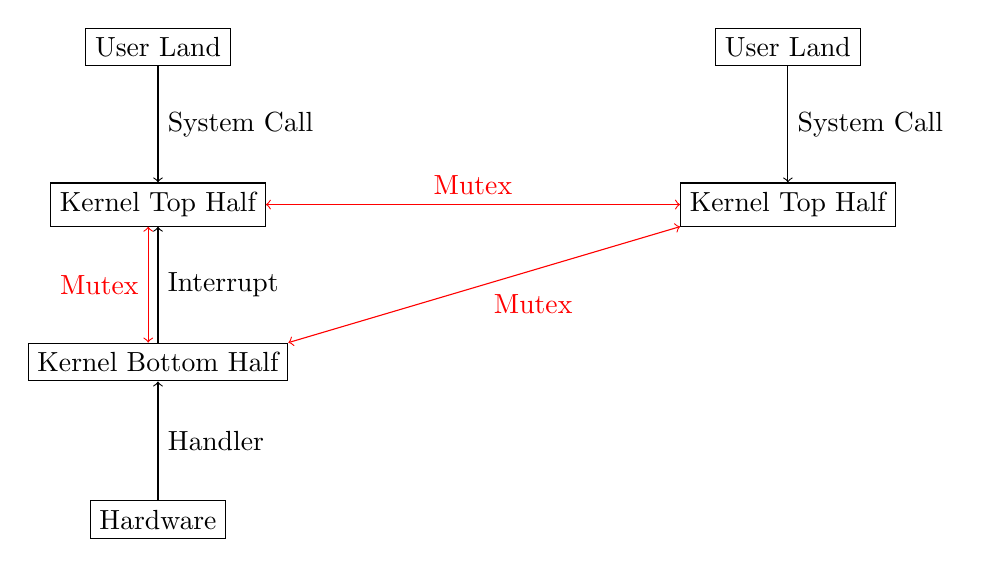
\begin{tikzpicture}
    \path (0, 2) node [draw] (ul) {User Land};
    \path (0, 0) node [draw] (to) {Kernel Top Half};
    \draw [->] (ul) -- (to) node[midway,right] {System Call};
    \path (0, -2) node [draw] (bo) {Kernel Bottom Half};
    \draw [<-] (to.south) -- (bo.north) node[midway,right] {Interrupt};
    \path (to.south) node (tos) {} (bo.north) node (bon) {};
    \draw [<->,red] (tos.west) -- (bon.west) node[midway,left,red] {Mutex};
    \path (0, -4) node [draw] (hw) {Hardware};
    \draw [<-] (bo) -- (hw) node[midway,right] {Handler};

    \path (8, 2) node [draw] (ul1) {User Land};
    \path (8, 0) node [draw] (to1) {Kernel Top Half};
    \draw [->] (ul1) -- (to1) node[midway,right] {System Call};

    \draw [<->,red] (to) -- (to1) node[midway,above] {Mutex};
    \draw [<->,red] (bo.north east) -- (to1.south west)
	node[midway, below right] {Mutex};
\end{tikzpicture}
\end{frame}

\subsection{Multi Processor Multi Queue}
\begin{frame}{Multi Processor Multi Queue}
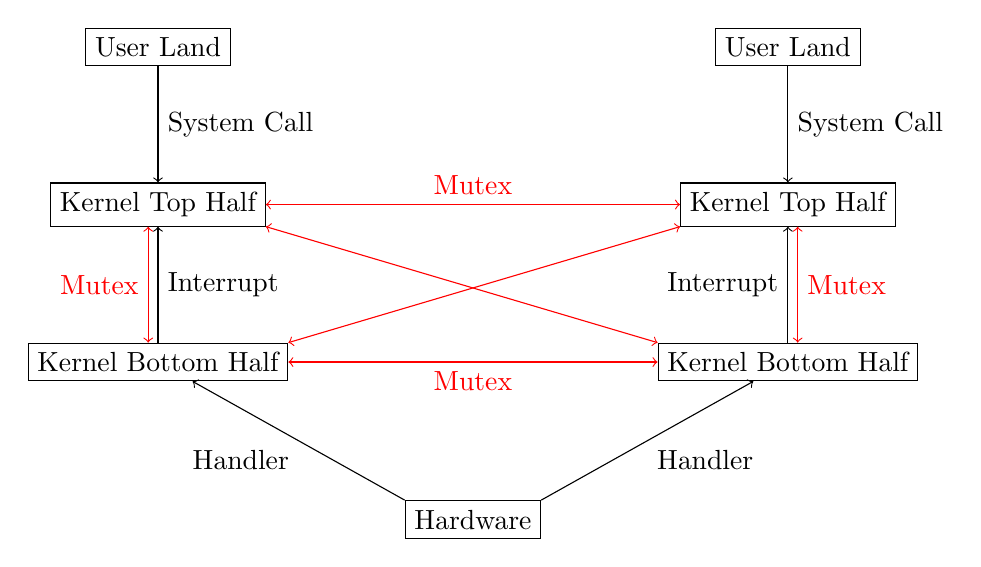
\begin{tikzpicture}
    \path (0, 2) node [draw] (ul) {User Land};
    \path (0, 0) node [draw] (to) {Kernel Top Half};
    \draw [->] (ul) -- (to) node[midway,right] {System Call};
    \path (0, -2) node [draw] (bo) {Kernel Bottom Half};
    \draw [<-] (to.south) -- (bo.north) node[midway,right] {Interrupt};
    \path (to.south) node (tos) {} (bo.north) node (bon) {};
    \draw [<->,red] (tos.west) -- (bon.west) node[midway,left,red] {Mutex};
    \path (4, -4) node [draw] (hw) {Hardware};
    \draw [<-] (bo) -- (hw.north west) node[midway,below left] {Handler};

    \path (8, 2) node [draw] (ul1) {User Land};
    \path (8, 0) node [draw] (to1) {Kernel Top Half};
    \draw [->] (ul1) -- (to1) node[midway,right] {System Call};
    \path (8, -2) node [draw] (bo1) {Kernel Bottom Half};
    \draw [<-] (to1.south) -- (bo1.north) node[midway,left] {Interrupt};
    \path (to1.south) node (tos1) {} (bo1.north) node (bon1) {};
    \draw [<->,red] (tos1.east) -- (bon1.east) node[midway,right,red] {Mutex};
    \draw [<-] (bo1) -- (hw.north east) node[midway,below right] {Handler};

    \draw [<->,red] (to) -- (to1) node[midway,above] {Mutex};
    \draw [<->,red] (bo.north east) -- (to1.south west)
	node[midway,below right] {};
    \draw [<->,red] (to.south east) -- (bo1.north west)
	node[midway,below right] {};
    \draw [<->,red] (bo) -- (bo1) node[midway,below] {Mutex};
\end{tikzpicture}
\end{frame}

\subsection{Kernel Threads}
\begin{frame}{Kernel Threads}
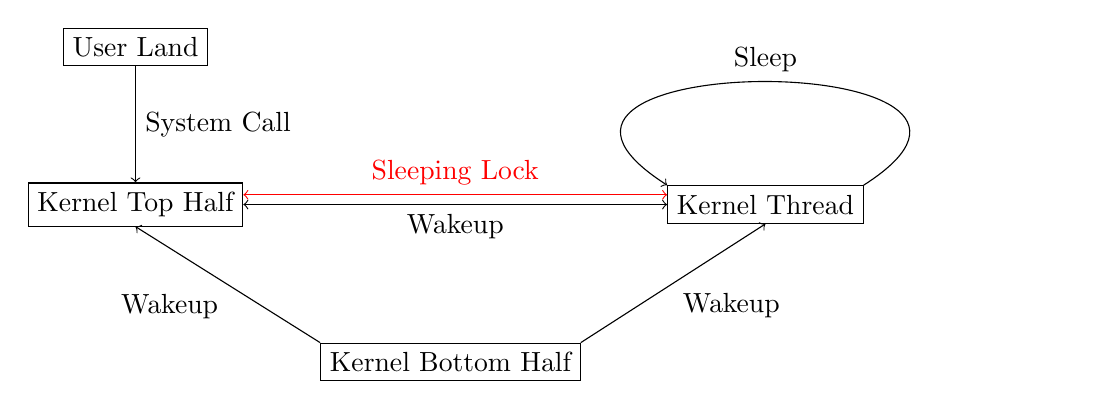
\begin{tikzpicture}
    \path (0, 2) node [draw] (ul) {User Land};
    \path (0, 0) node [draw] (to) {Kernel Top Half};
    \draw [->] (ul) -- (to) node[midway,right] {System Call};
    \path (4, -2) node [draw] (bo) {Kernel Bottom Half};
    \draw [<-] (to.south) -- (bo.north west) node[midway,below left] {Wakeup};

    \path (8, 0) node [draw] (kt) {Kernel Thread};
    \draw [->] (kt.north east) .. controls (12,2) and (4,2) ..  (kt.north west)
	node[midway,above] {Sleep};
    \draw [<-] (kt.south) -- (bo.north east) node[midway,below right] {Wakeup};
    \path (to.east) node (toe) {} (kt.west) node (ktw) {};
    \draw [<->,red] (toe.north) -- (ktw.north)
	node[midway,above] {Sleeping Lock};
    \draw [<->] (to.east) -- (kt.west) node[midway,below] {Wakeup};
\end{tikzpicture}
\end{frame}

\section{Network Stack}

\tikzset{
    queue/.pic={
	\path node [draw] (q1) {}
	    node [draw,right=0 of q1.east,anchor=west] (q2) {}
	    node [draw,right=0 of q2.east,anchor=west] (q3) {}
	    node [right=0 of q3.east,anchor=west] (q4) {\dots}
	    node [draw,right=0 of q4.east,anchor=west] (q5) {};
	\coordinate (-west) at (q1.west);
	\coordinate (-east) at (q5.east);
    }
}

\subsection{Softnet Receive}
\begin{frame}{Softnet Receive}
\begin{tikzpicture}
    \path (10, 2) node [draw] (ul) {User Land};
    \path (10, 0) node [draw] (sl) {Socket Layer};
    \path (7, -1) pic (sbq) {queue};
    \path (5, -2) node [draw] (st) {Softnet Thread};
    \path (2, -3) pic (ifq) {queue};
    \path (0, -4) node [draw] (ni) {Network Interrupt};

    \draw [->] (ni.north) |- (ifq-west) node [midway,above] {Interface Queue};
    \draw [->] (ifq-east) -| (st.south);
    \draw [->] (st.north) |- (sbq-west) node [midway,above] {Socket Buffer};
    \draw [->] (sbq-east) -| (sl.south);
    \draw [->] (ul) -- (sl) node [midway,right] {recv(2)};

    \path (st.north west) node (stnw) {};
    \draw [<->,red] (stnw.east) |- (sl.west) node[midway,above] {Net Lock};
\end{tikzpicture}
\end{frame}

\subsection{Softnet Send}
\begin{frame}{Softnet Send}
\begin{tikzpicture}
    \path (0, 2) node [draw] (ul) {User Land};
    \path (0, 0) node [draw] (sl) {Socket Layer};
    \path (2, -1) pic (sbq) {queue};
    \path (5, -2) node [draw] (st) {Softnet Thread};
    \path (7, -3) pic (ifq) {queue};
    \path (10, -4) node [draw] (ns) {Network Start};

    \draw [->] (ul) -- (sl) node [midway,right] {send(2)};
    \draw [->] (sl.south) |- (sbq-west)
	node [midway,below,label=below:(optional)] {Socket Buffer};
    \draw [->] (sbq-east) -| (st.north);
    \draw [->] (st.south) |- (ifq-west) node [midway,below] {Interface Queue};
    \draw [->] (ifq-east) -| (ns.north);

    \path (st.north east) node (stne) {};
    \draw [<->,red] (stne.west) |- (sl.east) node[midway,above] {Net Lock};
\end{tikzpicture}
\end{frame}

\subsection{Softnet Forwarding}
\begin{frame}{Softnet Forwarding}
\begin{tikzpicture}
    \path (0, -4) node [draw] (ni) {Network Interrupt};
    \path (1, -3) pic (ifiq) {queue};
    \path (5, -2) node [draw] (st) {Softnet Thread};
    \path (7, -3) pic (ifoq) {queue};
    \path (10, -4) node [draw] (ns) {Network Start};

    \draw [->] (ni.north) |- (ifiq-west) node [midway,above] {Interface Queue};
    \draw [<-] (st.south west) +(.5, 0) |- (ifiq-east);
    \draw [->] (st.south east) +(-.5, 0) |- (ifoq-west);
    \draw [->] (ifoq-east) -| (ns.north) node [midway,above] {Interface Queue};
\end{tikzpicture}
\end{frame}

\subsection{Configuration Lock}
\begin{frame}{Configuration Lock}
\begin{tikzpicture}
    \path (5, 2) node [draw] (if) {ifconfig};
    \path (5, 0) node [draw] (kc) {Kernel Config};
    \draw [->] (if) -- (kc) node [midway,right] {ioctl(2)};

    \path (0, -4) node [draw] (ni) {Network Interrupt};
    \path (1, -3) pic (ifiq) {queue};
    \path (5, -2) node [draw] (st) {Softnet Thread};
    \path (7, -3) pic (ifoq) {queue};
    \path (10, -4) node [draw] (ns) {Network Start};

    \draw [->] (ni.north) |- (ifiq-west) node [midway,above] {Interface Queue};
    \draw [<-] (st.south west) +(.5, 0) |- (ifiq-east);
    \draw [->] (st.south east) +(-.5, 0) |- (ifoq-west);
    \draw [->] (ifoq-east) -| (ns.north) node [midway,above] {Interface Queue};

    \path (kc.south) node (kcs) {} (st.north) node (stn) {};
    \draw [<-,red] (stn.west) -- (kcs.west)
	node [midway,left] {Exclusive Net Lock};
    \draw [->,red] (stn.east) -- (kcs.east)
	node [midway,right] {Shared Net Lock};
\end{tikzpicture}
\end{frame}

\subsection{Parallel Forwarding}
\begin{frame}{Parallel Forwarding}
\begin{tikzpicture}
    \path (0, -4) node [draw,label={[blue]right:x1,x4,x8}]
	(ni) {Network Interrupt};
    \path (1, -3) pic (ifiq) {queue};
    \path (5, -2) node [draw,label={[blue]below:x4}]
	(st) {Softnet Threads};
    \path (7, -3) pic (ifoq) {queue};
    \path (10, -4) node [draw,label={[blue]left:x1,x4,x8}]
	(ns) {Network Start};

    \draw [->] (ni.north) |- (ifiq-west) node [midway,above] {Interface Queue};
    \draw [<-] (st.south west) +(.5, 0) |- (ifiq-east);
    \draw [->] (st.south east) +(-.5, 0) |- (ifoq-west);
    \draw [->] (ifoq-east) -| (ns.north) node [midway,above] {Interface Queue};

    \path (2, -1) node [label={[blue]left:x4}] (ii) {ip\_input()};
    \path (5, -1) node (if) {ip\_forward()};
    \path (8, -1) node [label={[blue]right:x4}] (io) {ip\_output()};

    \draw (ii.south west) -- (st.north west);
    \draw (io.south east) -- (st.north east);
    \draw [->] (ii.east) -- (if.west);
    \draw [->] (if.east) -- (io.west);

    \draw [->] (ii) -- +(0, 1) node [anchor=south,label={[blue]above:x1}]
	{pf\_test()};
    \path (if) +(0, 1) node [anchor=south,label={[blue]above:x?}]
	(rt) {rtalloc()};
    \draw [->] (ii.north east) -- (rt.south west);
    \draw [->] (io) -- +(0, 1) node [anchor=south,label={[blue]above:x1}]
	{pf\_test()};
\end{tikzpicture}
\end{frame}

\subsection{Protocol Queue}
\begin{frame}{Protocol Queue}
\begin{tikzpicture}
    \path (9, 0) node [draw,label={[blue]right:x1}] (sl) {Socket Layer};
    \path (6.5, -1) pic (sbq) {queue};
    \path (6, -2) node [draw,label={[blue]right:x1}] (sp) {Softnet Proto};
    \path (3.5, -3) pic (ipq) {queue};
    \path (3, -4) node [draw,label={[blue]right:x4}] (si) {Softnet IP};
    \path (0.5, -5) pic (ifq) {queue};
    \path (0, -6) node [draw,label={[blue]right:x1,x4,x8}]
	(ni) {Network Interrupt};
    \draw [->] (ni.north) |- (ifq-west);
    \draw [->] (ifq-east) -| (si.south);
    \draw [->] (si.north) |- (ipq-west);
    \draw [->] (ipq-east) -| (sp.south);
    \draw [->] (sp.north) |- (sbq-west);
    \draw [->] (sbq-east) -| (sl.south);

    \path (sl.south west) node (slsw) {};
    \path (sp.north west) node (spnw) {};
    \draw [<->,red] (spnw.east) |- (slsw.north)
	node[midway,above] {Exclusive Net Lock};
    \path (si.north west) node (sinw) {};
    \draw [<->,red] (sinw.east) |- (sp.west)
	node[midway,above] {Shared Net Lock};
\end{tikzpicture}
\end{frame}

\subsection{Parallel Receive, UDP coming soon}
\begin{frame}{Parallel Receive, UDP coming soon}
\begin{tikzpicture}
    \path (10, 2) node [draw] (ul) {User Land};
    \path (10, 0) node [draw] (sl) {Socket Layer};
    \path (6.5, -1) pic (sbq) {queue};
    \path (3, -2) node [draw] (si) {Softnet IP};
    \path (si.east) node [draw,anchor=west,label={[blue]below:x4}]
	(sp) {Softnet Proto};
    \path (0.5, -3) pic (ifq) {queue};
    \path (0, -4) node [draw] (ni) {Network Interrupt};

    \draw [->] (ul) -- (sl);
    \path (ul.south) node (uls) {};
    \path (sl.north) node (sln) {};
    \draw [->] (uls.west) -- (sln.west);
    \draw [->] (uls.east) -- (sln.east) node [midway,right] {recv(2)};
    \draw [->] (ni.north) |- (ifq-west);
    \draw [->] (ifq-east) -| (si.south);
    \draw [->] (sp.north) |- (sbq-west);
    \draw [->] (sbq-east) -| (sl.south);

    \path (si.north west) node (sinw) {};
    \draw [<->,red] (sinw.east) |- (sl.west)
	node[midway,above] {Shared Net Lock};
    \path (sl.south east) node (slse) {};
    \draw [<->,red] (slse.west) |- (sp.east)
	node[near end,below] {per PCB Mutex};
\end{tikzpicture}
\end{frame}

\section{Performance Graphs}

\subsection{Weekly from 6.2 to 6.3}
\begin{frame}{Weekly from 6.2 to 6.3}
    \begin{adjustbox}{totalheight=\textheight-3\baselineskip}
	\input{gnuplot/2019-02-04T15:10:35Z-tcp.tex}
    \end{adjustbox}
\end{frame}



\section{How does it work?}

\begin{frame}{Agenda}
\setcounter{tocdepth}{1}
\tableofcontents[currentsection]
\end{frame}

\subsection{Performance Goals}
\begin{frame}{Performance Goals}
\begin{itemize}
    \item history
    \item reproducable
    \item details available
    \item drill down
    \item automatic
\end{itemize}
\end{frame}

\subsection{Performance History}
\begin{frame}{Performance History}
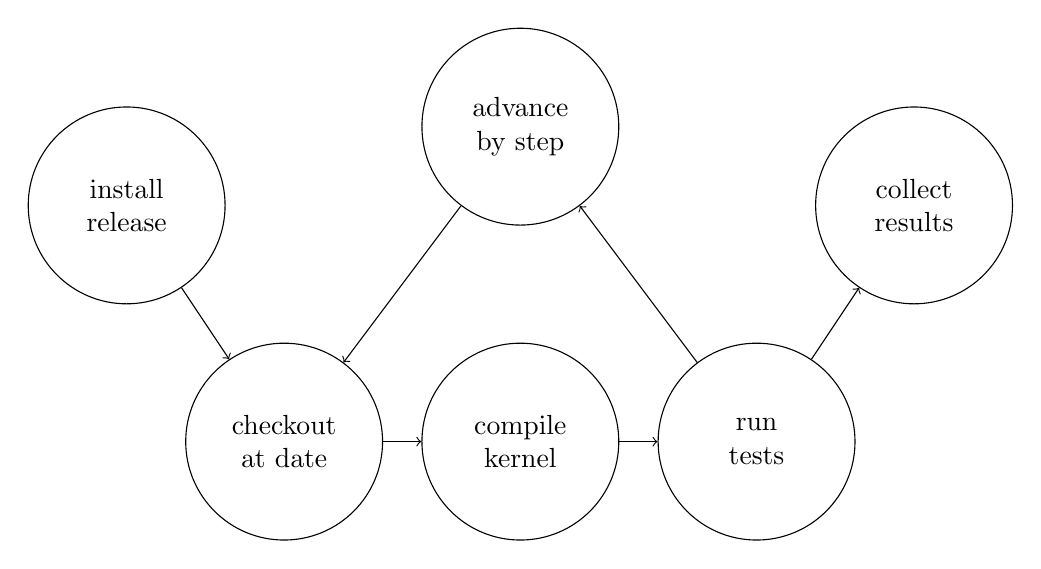
\begin{tikzpicture}
    \path ( 1, 1) node [draw,circle,align=center,minimum width=2.5cm]
	(release) {install\\release};
    \path ( 3,-2) node [draw,circle,align=center,minimum width=2.5cm]
	(checkout) {checkout\\at date};
    \path ( 6,-2) node [draw,circle,align=center,minimum width=2.5cm]
	(kernel) {compile\\kernel};
    \path ( 9,-2) node [draw,circle,align=center,minimum width=2.5cm]
	(test) {run\\tests};
    \path ( 6, 2) node [draw,circle,align=center,minimum width=2.5cm]
	(step) {advance\\by step};
    \path (11, 1) node [draw,circle,align=center,minimum width=2.5cm]
	(result) {collect\\results};
    \draw [->] (release) -- (checkout);
    \draw [->] (checkout) -- (kernel);
    \draw [->] (kernel) -- (test);
    \draw [->] (test) -- (result);
    \draw [->] (test) -- (step);
    \draw [->] (step) -- (checkout);
\end{tikzpicture}
\end{frame}

\subsection{Performance Hardware}
\begin{frame}{Performance Hardware}
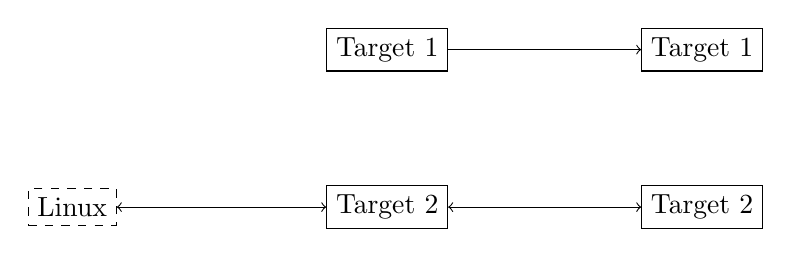
\begin{tikzpicture}
    \path (  0,   0) node [draw] (local1) {Target 1};
    \path (  4,   0) node [draw] (remote1) {Target 1};
    \draw [->] (local1) -- (remote1);
    \path (  0,  -2) node [draw] (local2) {Target 2};
    \path (  4,  -2) node [draw] (remote2) {Target 2};
    \draw [<->] (local2) -- (remote2);
    \path ( -4,  -2) node [draw,dashed] (linux) {Linux};
    \draw [<->] (linux) -- (local2);
\end{tikzpicture}
\end{frame}

\subsection{Performance Master}
\begin{frame}{Performance Master}
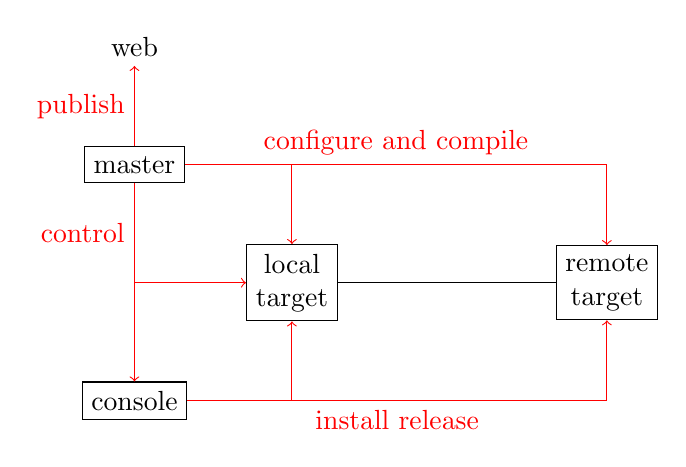
\begin{tikzpicture}
    \path ( -2,   3) node (web) {web};
    \path ( -2, 1.5) node [draw] (master) {master};
    \path ( -2,-1.5) node [draw] (console) {console};
    \path (  0,   0) node [draw,align=center] (local) {local\\target};
    \path (  4,   0) node [draw,align=center] (remote) {remote\\target};
    \draw (local) -- (remote);
    \draw [->,red] (master) -- (web) node [midway,left] {publish};
    \draw [->,red] (master) -- (console);
    \draw [->,red] (master) |- (local) node [near start,left] {control};
    \draw [->,red] (master) -| (local);
    \draw [->,red] (master) -| (remote)
	node [near start,above] {configure and compile};
    \draw [->,red] (console) -| (local);
    \draw [->,red] (console) -| (remote)
	node [near start,below] {install release};
\end{tikzpicture}
\end{frame}

\section{What are the findings?}

\begin{frame}{Agenda}
\setcounter{tocdepth}{1}
\tableofcontents[currentsection]
\end{frame}

\subsection{Reproduce and Reboot}
\begin{frame}{Reproduce and Reboot}
\begin{tikzpicture}
    \path ( 6,-2) node [draw,circle,align=center,minimum width=2.5cm]
	(kernel) {compile\\kernel};
    \path ( 9,-2) node [draw,circle,align=center,minimum width=2.5cm]
	(test) {run\\tests};
    \path (11,-4) node [draw,circle,align=center,minimum width=2.5cm]
	(keep) {run\\again};
    \path (14,-4) node [draw,circle,align=center,minimum width=2.5cm]
	(reboot) {reboot\\machine};
    \path (17,-4) node [draw,circle,align=center,minimum width=2.5cm]
	(reorder) {relink\\kernel};
    \draw [->] (checkout.east) -- (kernel);
    \draw [->] (kernel) -- (test);
    \draw [->] (test) -- (result);
    \draw [->] (test) -- (step);
    \draw [->] (test) -| (keep);
    \draw [->] (test) -| (reboot);
    \draw [->] (test) -| (reorder);
    \draw [->] (reorder) -- (reboot);
    \draw [->] (reboot) -- (keep);
    \draw [->] (keep) -| (test);
\end{tikzpicture}
\end{frame}

\subsection{Future Ideas}
\begin{frame}{Future Ideas}
\begin{itemize}
    \item forwarding throughput
    \item Linux client and server
    \item testing patches
    \item historic releases
    \item file system performance
\end{itemize}
\end{frame}

\subsection{Thanks}
\begin{frame}{Thanks}
\begin{itemize}
    \item Jan Klemkow for Hardware Administration
    \item Moritz Buhl for Visualization
    \item genua for Hosting and Worktime
\end{itemize}
\end{frame}

\subsection{Links}
\begin{frame}{Links}
\begin{itemize}
    \small
    \item \url{http://bluhm.genua.de/}
    \item \url{http://bluhm.genua.de/regress/results/regress.html}
    \item \url{http://bluhm.genua.de/perform/results/perform.html}
    \item \url{http://bluhm.genua.de/perform/results/gnuplot/test.data}
    \item \url{https://github.com/bluhm/regress-all}
    \item \url{https://github.com/bluhm/udpbench}
    \item \url{https://github.com/younix/testmaster}
    \item \url{https://github.com/bluhm/talk-perform}
\end{itemize}
\end{frame}

\subsection{Questions}
\begin{frame}{Questions}
\begin{center}
?
\end{center}
\end{frame}

\end{document}
